\section{Data retrieval process: gather and formatting social media data}

In this work it is proposed three datasets with social data from three social networks that are Twitter, Reddit and post blogs. Each dataset is build by using three different APIs: the Twitter API for the Twitter dataset, the Twingly API for the blog posts dataset and the Social Searcher API for the Reddit dataset. For each dataset, it is considered a set of keywords that will retrieve social information by exact matching in the corpus of each document. Since the retrieval must be performed for different languages, the keywords corresponds to named entities or specific lingo used in the social media in question. As it will be seen, some tweets were retrieved by using the special character \textit{\$} which denotes information related to the stock market.

\par The next sections are intended to explain the gathering process, how the data is formatted in order to persist it according to legal concerns of the social media source information and some limitations related to the use of these type of APIs and the information they provide.
\subsection{Gathering process}
%APIS: Twitter, Twingly and Social Media Searcher
Typically, in the gathering process of any type of social data is implied the time variable which, for example,  can be used to cluster documents by fixed window times. The building process of the different datasets provided comprise periods of time in terms of its retrieval. The table \ref{table:periodTime} shows the dates when the retrieval process starts and ends per dataset.

\begin{table}[htb]
	\begin{center}
		\begin{tabular}{|l|r|r|}
			\hline
			\textbf{Dataset} &    \textbf{Start date } &\textbf{ End date}\\
			\hline \hline
			Twitter              &  2021-12-04  &  2021-12-31\\ 
			\hline
			Blog posts &  2021-11-08 	& 2021-12-06 \\
			\hline
			Reddit &  2021-11-08   	& 2021-12-06 \\
			\hline
		\end{tabular}
	\end{center}
	\caption{Start and end dates of the retrieval data}
	\label{table:periodTime}
\end{table}

Each dataset is built according to a fixed set of keywords that corresponds to named entities. Each keyword belongs to the domain of music, stock market, news related to a natural disaster, technology and influencers. The table \ref{table:keywords} summarizes this information.\\

%Social media considered, Keywords (named entities), gathering time window.
\begin{table}[h]
	\centering
	\begin{tabular}{|c|c|c|c|c|}
		\hline
		\textbf{Keyword} & \textbf{Domain} & \multicolumn{3}{c|}{\textbf{Dataset}} \bigstrut\\
		\hline \hline
		\textit{paramore} & \multirow{3}[6]{*}{Music} & \multirow{14}[28]{*}{Twitter} & \multirow{7}[14]{*}{Blog posts} & \multirow{6}[12]{*}{Reddit} \bigstrut\\
		\cline{1-1}    \textit{my chemical romance} &       &       &       &  \bigstrut\\
		\cline{1-1}    \textit{the smashing pumpkins} &       &       &       &  \bigstrut\\
		\cline{1-2}    \textit{la palma} & News  &       &       &  \bigstrut\\
		\cline{1-2}    \textit{dalas} & Influencer &       &       &  \bigstrut\\
		\cline{1-2}    \textit{apple} & \multirow{2}[4]{*}{Technology} &       &       &  \bigstrut\\
		\cline{1-1}\cline{5-5}    \textit{microsoft} &       &       &       & \multirow{8}[16]{*}{} \bigstrut\\
		\cline{1-2}\cline{4-4}    \textit{\$AMC} & \multirow{7}[14]{*}{Financial} &       & \multirow{7}[14]{*}{} &  \bigstrut\\
		\cline{1-1}    \textit{\$GME} &       &       &       &  \bigstrut\\
		\cline{1-1}    \textit{\$AAPL} &       &       &       &  \bigstrut\\
		\cline{1-1}    \textit{\$HOOD} &       &       &       &  \bigstrut\\
		\cline{1-1}    \textit{\$MSFT} &       &       &       &  \bigstrut\\
		\cline{1-1}    \textit{\$NVDA} &       &       &       &  \bigstrut\\
		\cline{1-1}    \textit{\$TWKS} &       &       &       &  \bigstrut\\
		\hline
	\end{tabular}%
	\label{table:keywords}%
	\caption{Keywords with their domain and datasets containing them.}
\end{table}%
\par 
For each day in the periods of time described in Table \ref{table:periodTime} a daily retrieval process was executed. For the Twitter dataset, it was retrieved 100.000 tweets per day. The blog posts dataset was built only with a single API call since Twingly indexes articles and stores them in their database and the API call retrieves information persisted from the three lasts months.
However, for the Reddit dataset only 100 posts could be retrieve without taking into account of repeated posts.
\subsection{Formatting process}
The three APIs used to retrieve the social data define a set of properties returned in the response of the API call. However, not all information is considered in the dataset building process for legal or practical reasons. In the gathering and processing the Twitter information the textual information must be deleted because the Twitter terms and conditions of its API usage. It is important to remark that with the tweet ID or the user ID it can be retrieved more information provided by the Twitter API. In this work, it will be only considered these IDs and the date and language of each tweet. The following schema defines the structure of a tweet in the dataset.
%Tweet
\begin{figure}[H]
	\begin{Verbatim}[xleftmargin=.5in]
		// Tweet format
		{
			"date": ,
			"id_tweet": ,
			"language": ,
			"user_id": 
		}
	\end{Verbatim}
	\caption{Structure of a retrieved tweet.}
\end{figure}


\par 

The Reddit dataset contains information about the sentiment of the text and popularity information related to the number of likes and comments of each post. the Figure \ref{fig:twinglyStructure} shows the schema for a persisted Reddit post in the dataset.
\begin{figure}[H]
	\begin{Verbatim}[xleftmargin=.5in]
		{
			// Reddit document format
			"post_id": ,
			"lang": ,
			"date_posted": ,
			"sentiment": ,
			"text": ,
			"ups": ,
			"comments": ,
			"user_name": ,
			"user_id": ,
			"user_url": 
		}
	\end{Verbatim}
	\caption{Structure of a Reddit post.}
	\label{fig:redditStructure}
\end{figure}

\par

Lastly, the Twingly API was used to retrieve the blog posts information regarding the keywords and languages considered. In comparison with the later structures, Twingly provides more information like the images attached for each post or the links contained. The blog post structure is depicted in the Figure \ref{fig:twinglyStructure}.
%Blog posts
\begin{figure}[H]
	\begin{Verbatim}[xleftmargin=.5in]
		// Blog post document format
		{
			"author": ,
			"authority": ,
			"blog_id": ,
			"blog_name": ,
			"blog_rank": ,
			"blog_url": ,
			"coordinates": ,
			"id": ,
			"images": ,
			"indexed_at": ,
			"inlinks_count": ,
			"language_code": ,
			"latitude": ,
			"links": ,
			"location_code": ,
			"published_at": ,
			"reindexed_at": ,
			"tags": ,
			"text": ,
			"title": ,
			"url"
		}
	\end{Verbatim}
	\caption{Structure of a blog post}
	\label{fig:twinglyStructure}
\end{figure}
\subsection{Limitations}

The Twitter API limits the number of API calls per day. This led to the retrieval process to take several hours because wait clauses must be coded to avoid the rejection of API calls by the Twitter side. Furthermore, the textual information can not be shared publicly due to legal Twitter concerns. However, with the tweet ID it is possible to retrieve the metadata that defines a tweet such that the geographical position where the tweet was posted, the number of retweets etc. \\

\par Twingly provides a great API to retrieve blog posts. However, the supported format is XML which is not the trend nowadays. Nonetheless, there exists packages that allow to translate files from XML to JSON format.
\par Lastly, the Social Searcher API is the most restrictive. Only 100 posts per API call can be retrieved and the language of the posts is not guaranteed to match with the one specified in the API call. However, the API response contains attributes that can be exploited in the sentiment analysis context like the sentiment property.
%Reddit

\newpage
\section{Data analysis}



% Questions that motivates the analysis
The data analysis consists in study frequentist information derived from the data considered in the data structures commented. This analysis is done at two levels regarding the persisted information: (1) At dataset level where it is reflected how varies the number of posts in function the language and the date posted; (2) At named entity level where it is studied each dataset in function the specific characteristic of the dataset. I.e the number of hashtags per named entity per named entity.
\subsection{Corpora analysis at dataset level}

\subsubsection{Twitter dataset analysis}
\begin{figure}[H]
	\begin{center}
		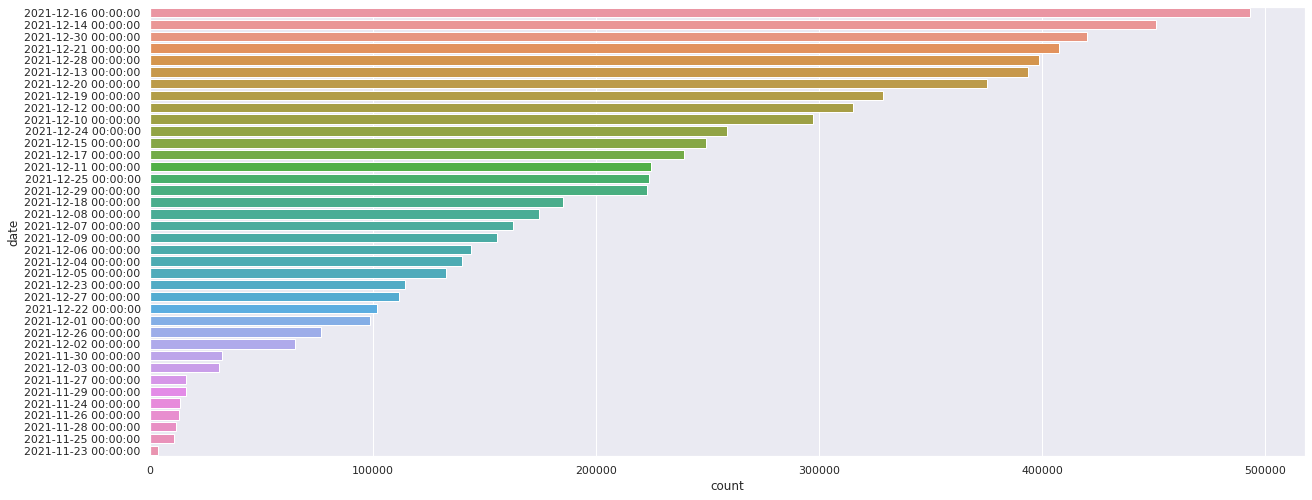
\includegraphics[scale=0.35]{twitter/datasetlevel/twitter_postcounts_date.png}
		\caption{Number of tweets published per date. Only the dates with higher values are shown.}
		\label{fig:twitter_postcounts_date}
	\end{center}
\end{figure}

\begin{figure}[H]
	\begin{center}
		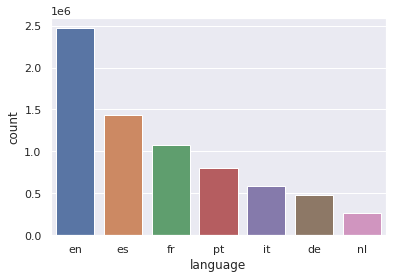
\includegraphics[scale=0.5]{twitter/datasetlevel/twitter_postcounts_lang.png}
		\caption{Tweet count posted per language.}
		\label{fig:twitter_postcounts_lang}
	\end{center}
\end{figure}
\subsubsection{Blog post dataset analysis}

\begin{figure}[H]
	\begin{center}
		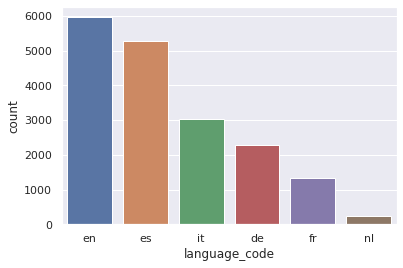
\includegraphics[scale=0.5]{blogposts/datasetlevel/blogpost_postcounts_lang.png}
		\caption{Blog post count posted per language.}
		\label{fig:blogpost_postcounts_lang}
	\end{center}
\end{figure}

\begin{figure}[H]
	\begin{center}
		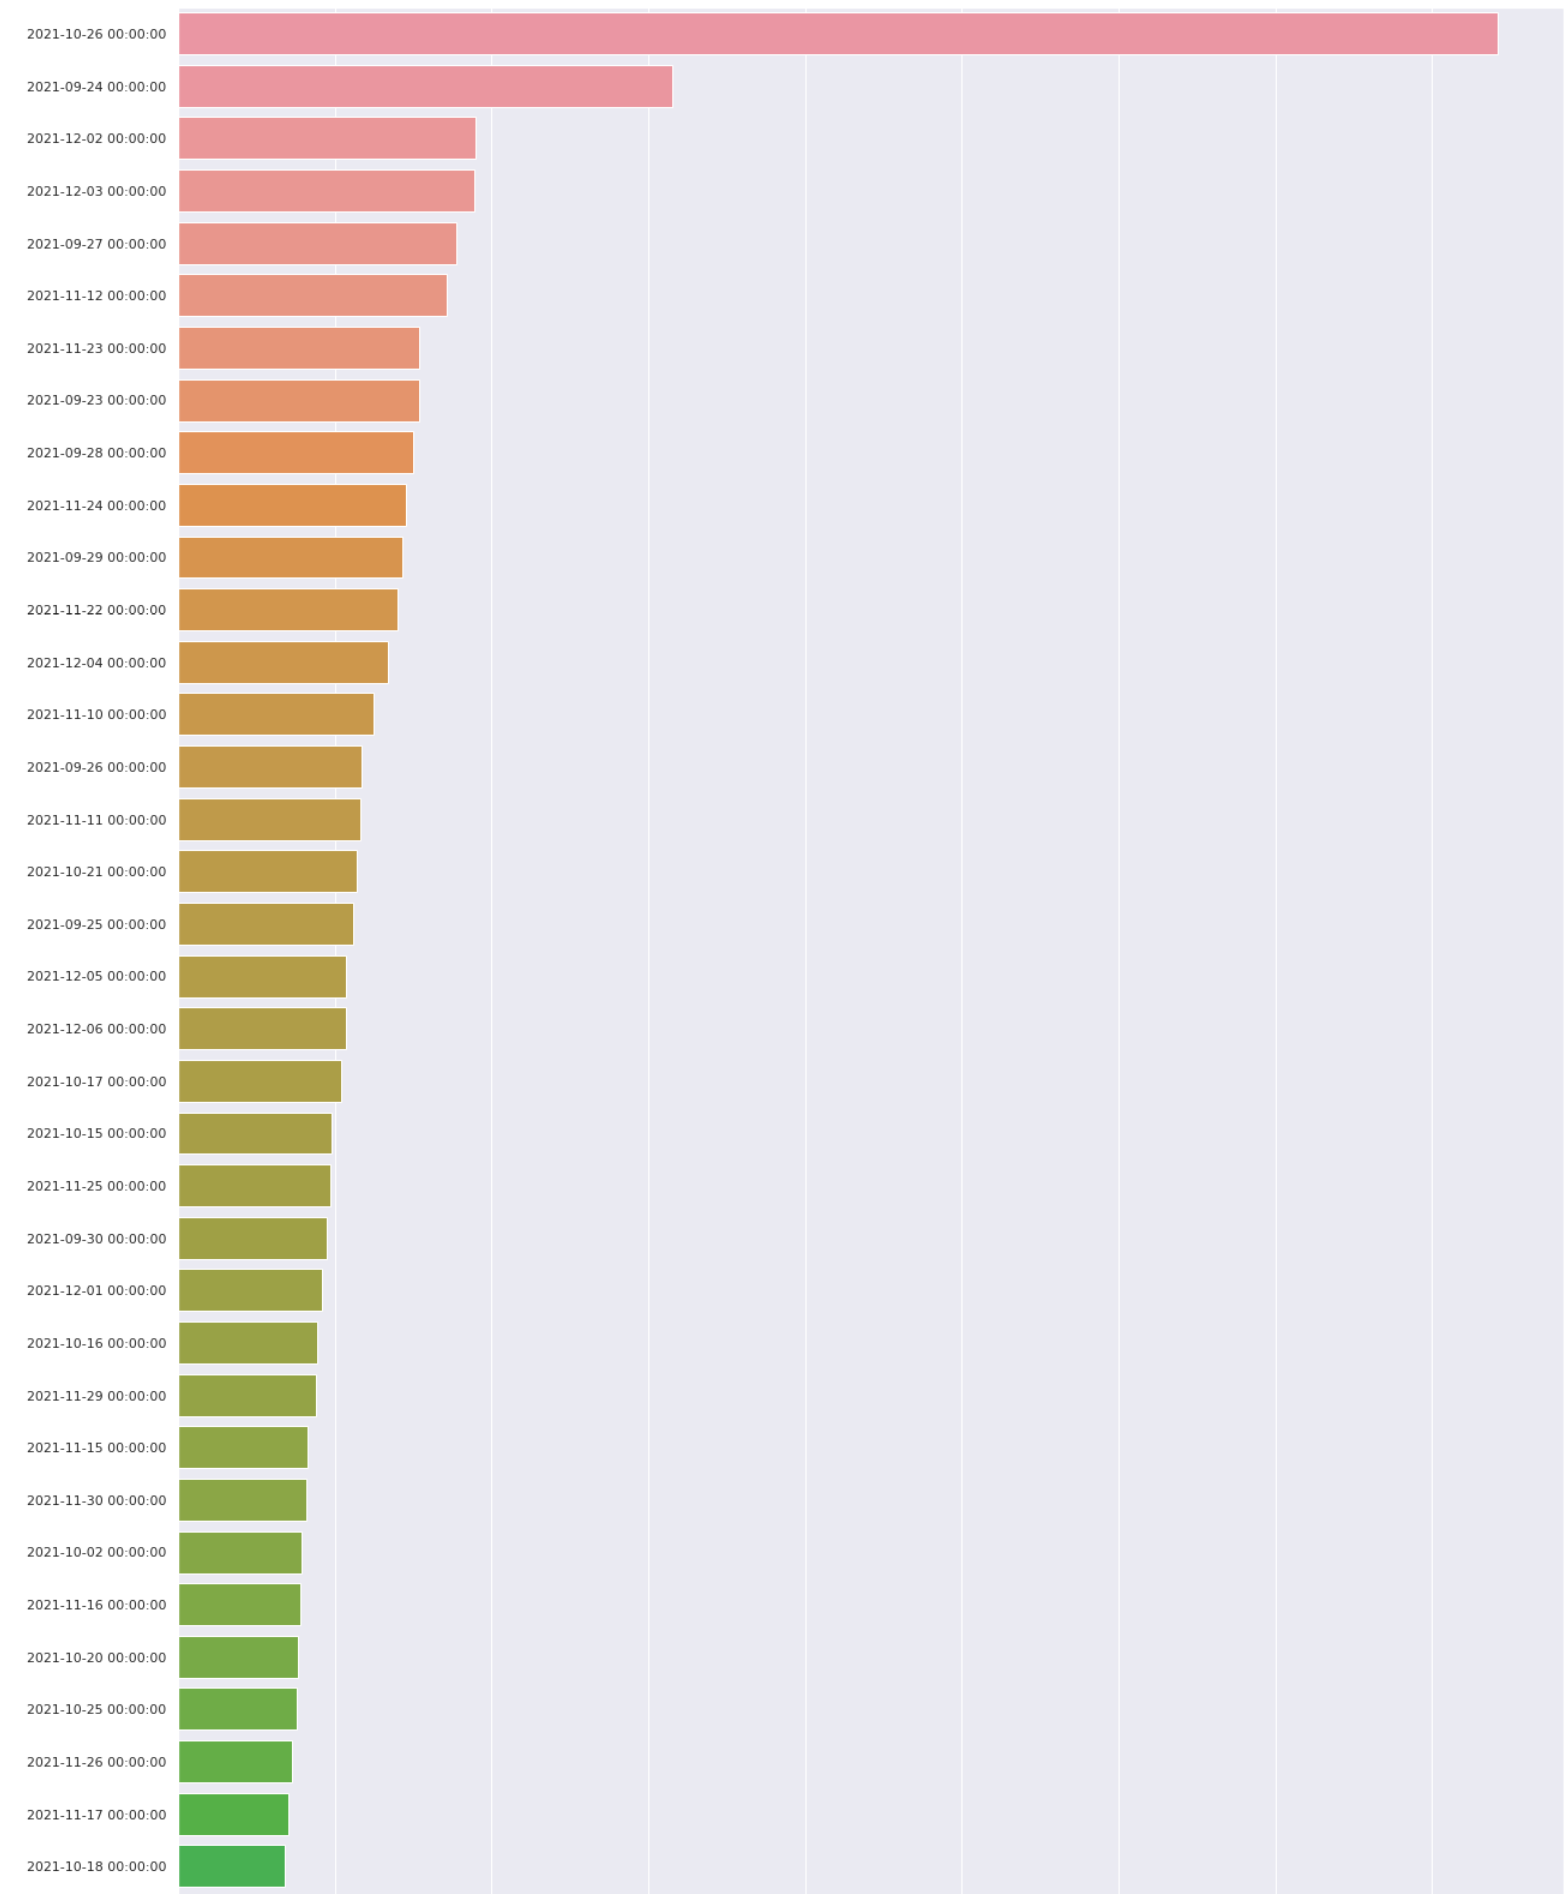
\includegraphics[scale=0.5]{blogposts/datasetlevel/blogpost_postcounts_date.png}
		\caption{Blog post count posted per date. Only the dates with higher values are shown.}
		\label{fig:blogpost_postcounts_date}
	\end{center}
\end{figure}


\subsubsection{Reddit dataset analysis}

\begin{figure}[H]
	\begin{center}
		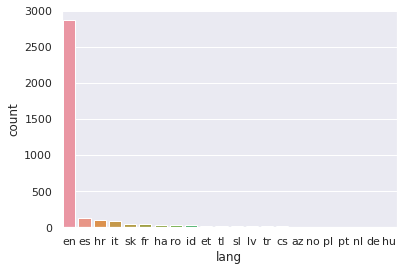
\includegraphics[scale=0.5]{reddit/datasetlevel/reddit_postcounts_lang.png}
		\caption{Reddit post count posted per language.}
		\label{fig:reddit_postcounts_lang}
	\end{center}
\end{figure}

\begin{figure}[H]
	\begin{center}
		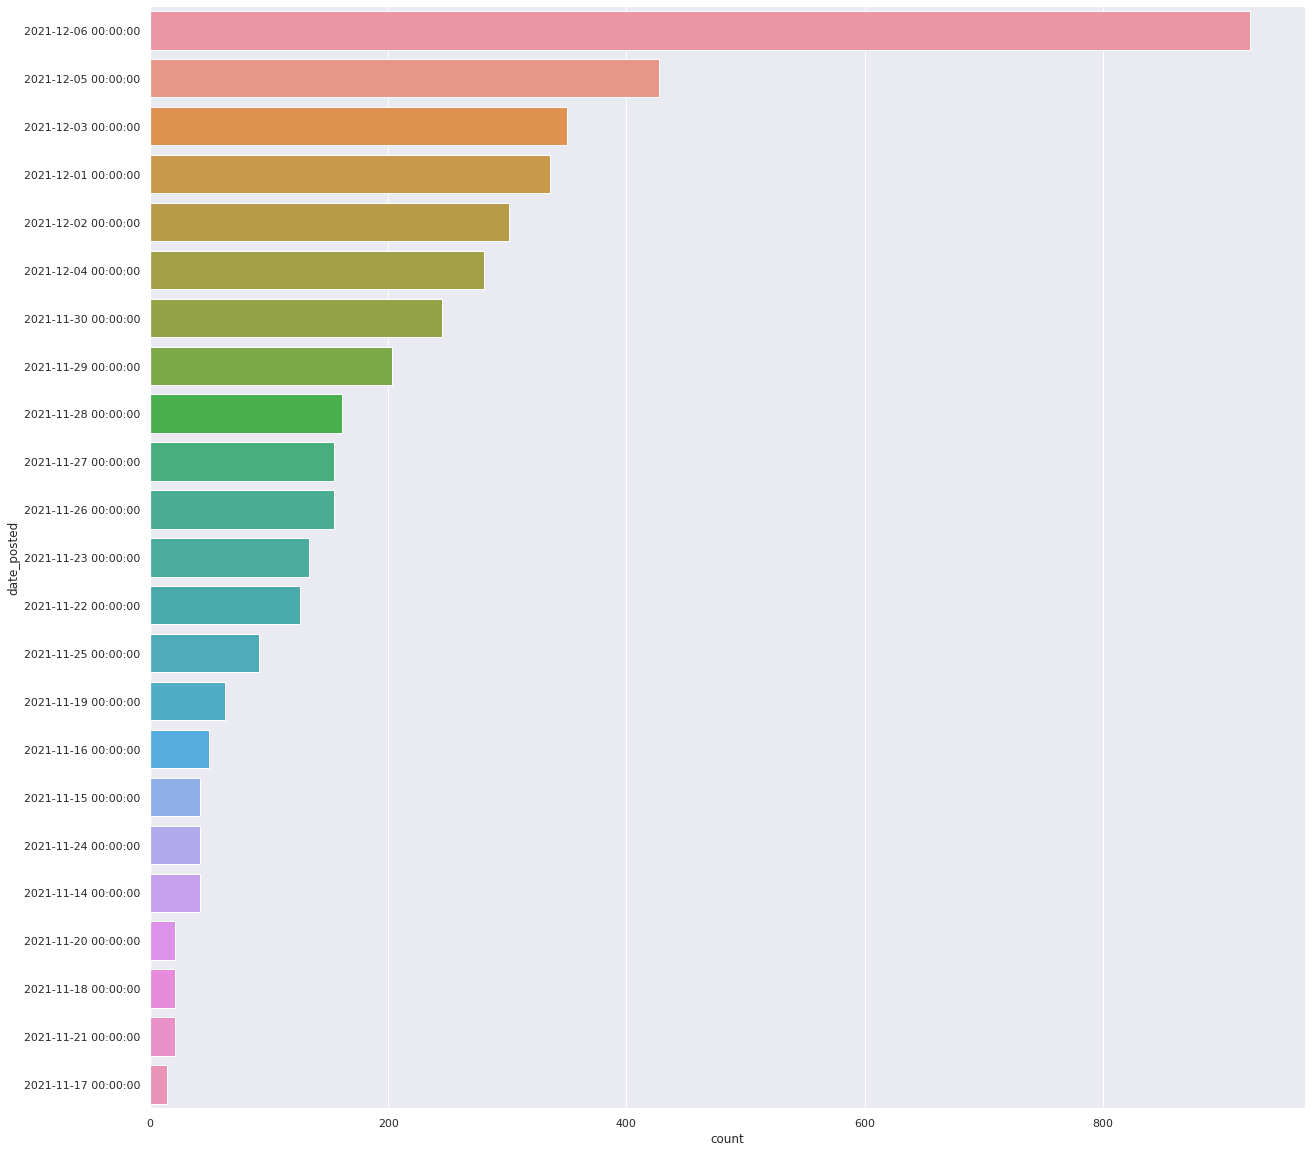
\includegraphics[scale=0.3]{reddit/datasetlevel/reddit_postcounts_date.png}
		\caption{Reddit post count posted per date. Only the dates with higher values are shown.}
		\label{fig:reddit_postcounts_date}
	\end{center}
\end{figure}

% 
%TODO include captures
%TODO explain each one
\subsection{Corpora analysis at named entity level}
\subsubsection{Twitter dataset analysis}
\subsubsection{Blog post dataset analysis}
\subsubsection{Reddit dataset analysis}

%TODO include captures
%TODO explain each one
% Copora analysis at dataset level
	% Number of posts of each social media
	% Number of posts of each language an social media
	% Distribution of links of each social media
	
% Corpora analysis at named entity level
	% Twitter 
		% # hashags containing the named entity
		% # links
		% # Rt's
		% Number of posts published per day
		
	% Reddit

		% average ups per entity (or box plot)
		% average comments per entity (or boxplot)
		% Number of negative and positive reddits posts
		% # posts per language
	%Twingly posts
		% Distribution of number of posts for each language
		% Distribution of number of posts with links
		% Number of posts published per day
		% Average number of tags
		% Average length of text and title
		% 
